\chapter{Premières manipulations du graphe}
Une fois la transformation en graphe de nos données achevée, on doit les stocker dans une base de données pour les exploiter. Dans le projet c'est le logiciel de base de graphes GraphDB Free\footnote{Voici le lien du site. \href{https://graphdb.ontotext.com/}{https://graphdb.ontotext.com/}} qui a été utilisé. Il s'agit d'une base de graphes sémantiques, ce type de base de données (autrement appelé \textit{triplestore}) est spécialisé dans le langage RDF. De tels logiciels mettent à disposition des outils pour mieux interagir avec les données et les comprendre. Une fois chargées, les données peuvent être interrogées de différentes manières et peuvent même être modifiées, le tout à l'aide du langage SPARQL.
\section{L'intérêt d'un triplestore}
\subsection{Le choix de GraphDB}
Pour l'extension de la preuve de concept nous avons eu besoin d'un triplestore facile à prendre en main et léger. Le logiciel GraphDB remplit ces deux exigences. Développé par la société Ontotext, spécialisée dans les technologies du Web Sémantique, ce triplestore est disponible sous deux éditions, une gratuite et une payante. Bien qu'ayant certaines limitations, l'édition GraphDB Free est largement suffisante pour un projet de notre taille. Elle est développée en Java, et pour aller plus loin dans la configuration il faudra au minimum quelques notions sur ce langage, mais nous n'en avons pas eu besoin pour l'instant. Une instance de Graph DB Free peut être installée et fonctionner sur un ordinateur en local, ce qui a été très pratique pour expérimenter facilement un échange de requêtes entre le SPARQL Endpoint\footnote{Un SPARQL Endpoint est un point d'accès d'un triplestore qui permet d'envoyer des requêtes SPARQL au format HTTP afin d'interroger la base de données à partir d'un client.} mis à disposition par GraphDB et l'interface de recherche que nous présenterons dans le chapitre suivant. L'interface GraphDB met également à disposition des visualisations bien pratiques pour appréhender la quantité de relations entre classes. (voir annexe \ref{fig:visualisation-classe-graphdb}\label{chapitre6})
\subsection{L'inférence sur les données}
Un des intérêts d'un triplestore vient du principe qu'il sait interpréter les langages RDFS et OWL, utilisés pour construire une ontologie et qui permettent de spécifier pour ses composants des propriétés permettant d'inférer des faits. Une fois chargées dans la base les ontologies RiC-O et ORESM, Graph DB Free va raisonner sur les triplets qui sont importés et va créer à partir de chaque triplet d'autres triplets déduits de la logique formelle de l'ontologie. C'est ce qu'on appelle l'inférence. Dans l'ontologie, la hiérarchie des classes (et même des relations) implique que si la classe A est une sous-classe de la classe B alors une entité de la classe A est également une entité de la classe B. C'est ce à quoi sert la super classe \textbf{Thing}\footnote{\href{https://www.ica.org/standards/RiC/ontology\#Thing}{https://www.ica.org/standards/RiC/ontology\#Thing}} ou la relation \textbf{is related to}\footnote{\href{https://www.ica.org/standards/RiC/ontology\#isRelatedTo}{https://www.ica.org/standards/RiC/ontology\#isRelatedTo}}, on va du plus général au plus précis dans la hiérarchie, et le triplestore le comprend. Si nous prenons le cas d'une personne, dans nos données transformées :  il a été choisi que les personnes seraient représentées par la classe rico:Person, iIl y a donc dans nos fichiers le triplet explicite : "l'URI de la personne" -> rdf:type -> rico:Person. Mais puisque l'ontologie définit que la classe Person est une sous-classe de la classe \textbf{Agent}\footnote{\href{https://www.ica.org/standards/RiC/ontology\#Agent}{https://www.ica.org/standards/RiC/ontology\#Agent}}, qui elle-même est une sous classe de la classe \textbf{Thing} alors le triplestore au moment du chargement de l'entité dans la base va également produire deux nouveaux triplets par inférence\footnote{Graph DB appelle ces triplets des triplets implicites.}, qui seront : "l'URI" -> rdf:Type -> rico:Agent et l'autre rico:Thing. Ce système permet de gérer la granularité des requêtes sur la base. Si l'on veut extraire des données générales on peut utiliser les super classes ou les super relations. Cela ouvre de grandes possibilités de raisonnement, mais encore faut il bien maîtriser le modèle de données pour l'interroger efficacement.
\par
Les autres triplets inférés viennent de la définition de certaines relations. Comme nous l'avions évoqué, toutes les relations dans notre ontologie (à l'exception des relations symétriques) ont des relations inverses.\par
Faisons une analogie avec un fait du monde réel. Pour exprimer le fait qu'un homme est le père de son fils, on pourrait imaginer la relation \textbf{est parent de}. De ce simple fait on peut déduire la relation entre l'enfant et son père, qui pourrait être représentée par \textbf{est enfant de}. Les deux relations sont inverses l'une de l'autre. Si l'une est exprimée dans un jeu de données on doit pouvoir inférer l'autre.
\par
C'est la même chose pour notre ontologie, prenons l'exemple de la relation \textbf{has author}\footnote{\href{https://www.ica.org/standards/RiC/ontology\#hasAuthor}{https://www.ica.org/standards/RiC/ontology\#hasAuthor}} fournie par RiC-O, elle lie un document à son auteur, et bien cette relation a pour inverse \textbf{is author of}\footnote{\href{https://www.ica.org/standards/RiC/ontology\#isAuthorOf}{https://www.ica.org/standards/RiC/ontology\#isAuthorOf}}. Pour tout les cas comme celui-ci, cela permet de ne devoir indiquer la relation que dans un sens. Le moteur d'inférence de la base de graphes inférera le triplet inverse. D'autres caractéristiques peuvent être données à des relations qui produiront d'autres triplets par inférence. On peut citer une relation symétrique\footnote{Une relation symétrique implique le même triplet en échangeant de position le sujet et l'objet.}.
\par
L'inférence permet deux choses, dans un premier lieu de simplifier la construction des données initiales dans lesquelles on peut se permettre de ne produire les relations que dans un seul sens. Pour notre cas, lors de la transformation de nos données nous avons créé 87 000 triplets, en chargeant nos données dans le triplestore, celui-ci a ajouté presque 220 000 triplets. Environs trois triplets sur quatres viennent de l'inférence sur nos données.  L'inférence permet également d'améliorer la recherche en permettant d'avoir davantage de triplets et donc davantage de manières d'entrer et de naviguer dans le graphe. Pour interroger et visualiser ce graphe, deux outils complémentaires sont mis à disposition par GraphDB.
\section{Interrogation des données}
\subsection{Visualisation}
La première méthode proposée pour explorer nos données est visuelle. On peut explorer à partir de l'interface GraphDB une partie du graphe représentant nos données. A partir d'un URI, on pénètre dans le graphe et on navigue. C'est très utile pour cibler certaines entités et voir leurs interactions. Cette visualisation graphique montre clairement le changement de nature des données. Il est aisé de naviguer de nœud en nœud pour parcourir les données, et l'utilisation de couleurs différentes pour représenter les classes rend aisée la lecture. C'est un outil idéal quand on veut interroger le graphe simplement sur un élément précis. Mais cette visualisation a ses limites, dès lors que le graphe contient un grand nombre de triplets. Pour tous les interroger, on ne peut pas se contenter d'un tel dispositif. Ci-dessous vous pouvez voir les lignes 1 et 2 du tableau du collège de Hubant, initialement dans les tableaux de dépouillement et après leur visualisation sous forme de graphe.
\begin{figure}[!h]
    \centering
    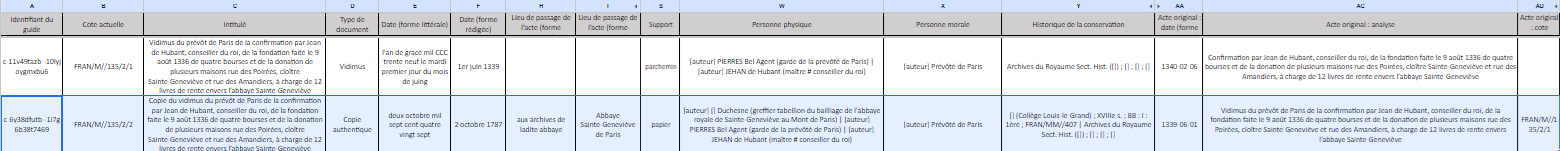
\includegraphics[width=1.14\linewidth]{images/ligne tableau.png}
    \caption{Ligne 1 et 2 du tableau de dépouillement du collège de Hubant.}
    \label{fig:tableau-depouillement-hubant}
\end{figure}
\begin{figure}[!h]
    \centering
    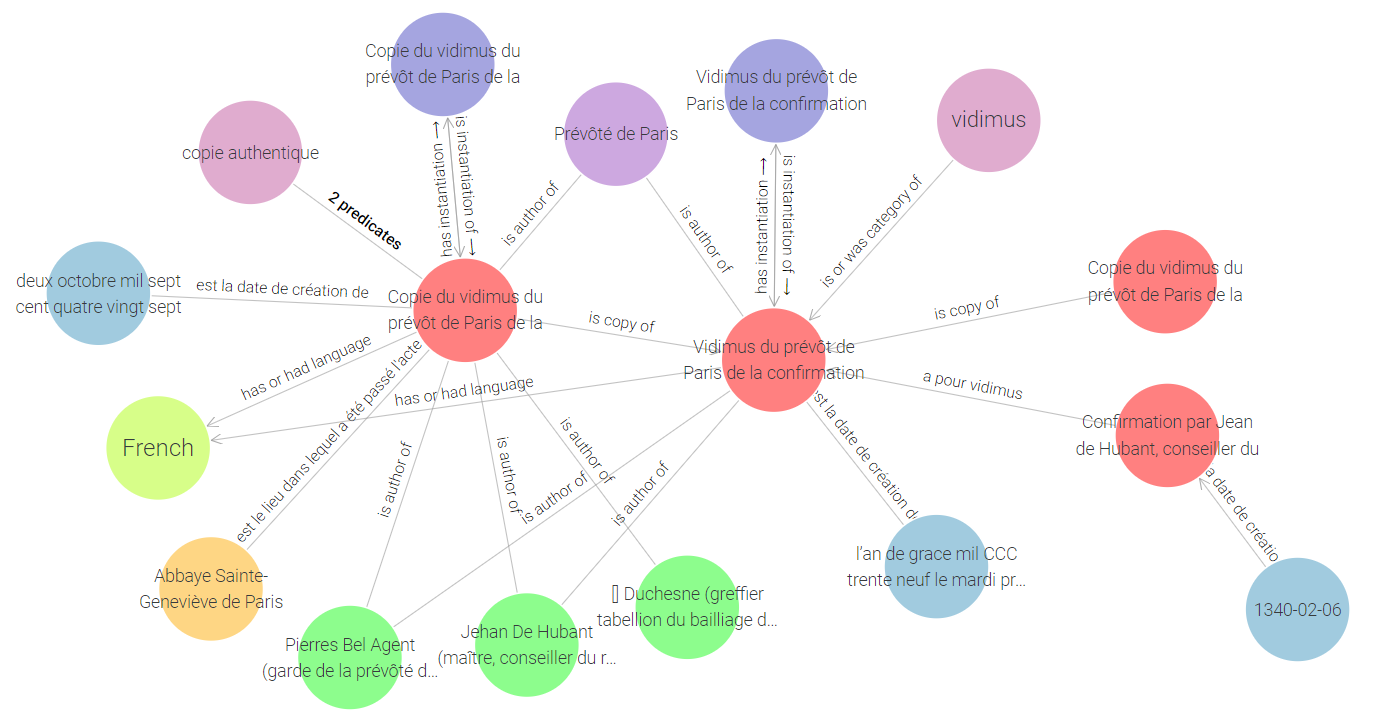
\includegraphics[width=0.9\linewidth]{images/visiualisation graphe hubant.png}
    \caption{Visualisation en graphe, de ces mêmes lignes transformées en RDF, centrée sur les RecordResource.}
    \label{fig:graphe-hubant}
\end{figure}
\subsection{SPARQL}
La seconde méthode consiste à utiliser l'éditeur de requête SPARQL. SPARQL (SPARQL Protocol and RDF Query Language) est un langage de requête spécifiquement conçu pour interroger les données RDF. Il offre une syntaxe expressive et puissante, permettant de formuler des requêtes complexes pour extraire des informations précises et pertinentes. De plus, il permet d'effectuer des requêtes distribuées, ce qui signifie qu'il peut interroger des sources multiples réparties dans le Web de données et ainsi permettre leur agrégation. Pour faciliter l'écriture des requêtes, SPARQL permet la déclaration de préfixes\footnote{Pour RiC-O ce préfixe (qui est déclaré dans l'ontologie) est \textbf{rico}, pour l'ontologie ORESM c'est \textbf{oresm-onto}.} qui remplacent la partie invariante des URIs\footnote{La partie invariante des URIs des composants de RiC-O est <https://www.ica.org/standards/RiC/ontology\#>.} d'une ontologie.
\begin{figure}[!h]
    \centering
    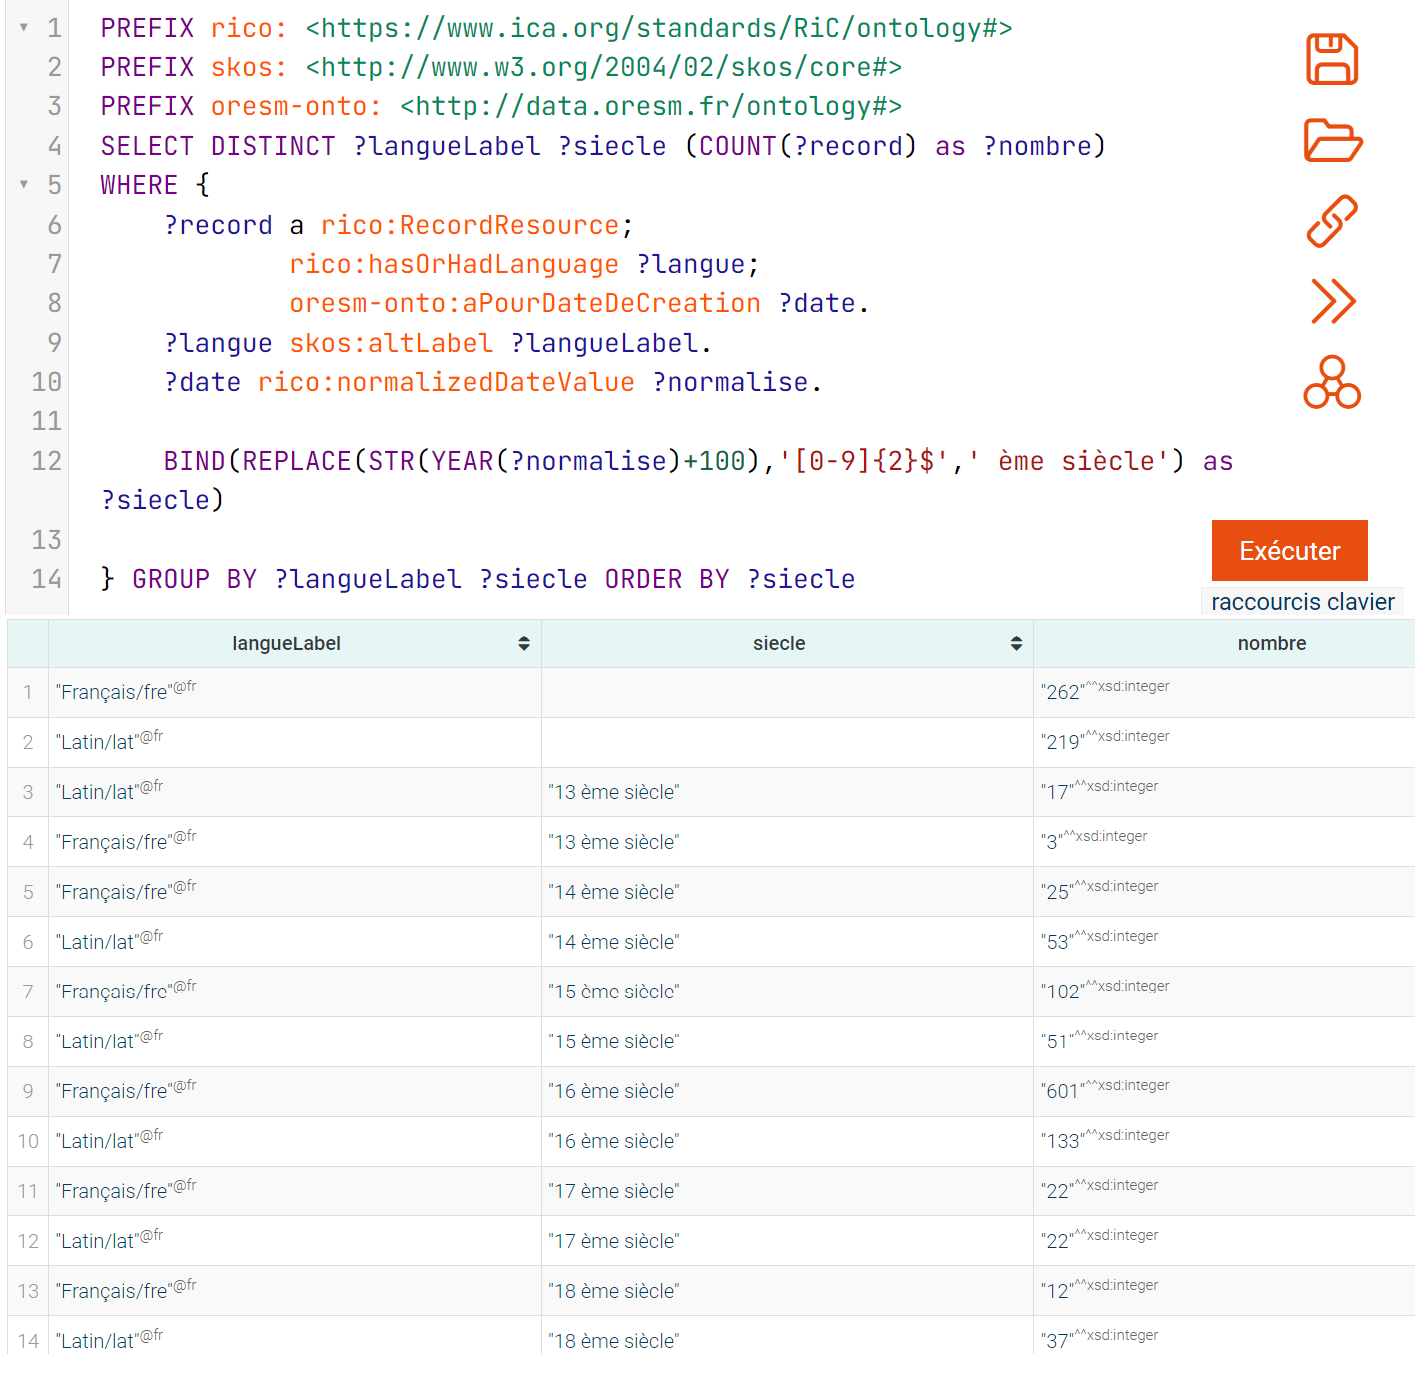
\includegraphics[width=0.95 \linewidth]{images/requete sparl langue resultat.png}
    \caption{Un exemple de requête SPARQL dans l'interface GraphDB et le résultat associé.}
    \label{fig:sparql_requete}
\end{figure}

Dans la requête d'exemple ci-dessus on opère une recherche sur les données. C'est le rôle du mot clé \textbf{SELECT}. SPARQL fonctionne en utilisant des variables, chaque variable peut être sujet, prédicat et/ou objet d'un triplet. Les résultats contiennent les valeurs que les variables contiennent quand l'ensemble des triplets dans la clause \textbf{WHERE} sont possibles. On peut également appliquer un traitement sur les données littérales, comme, dans l'exemple, avec des expressions régulières ou des opérations mathématiques, et on peut par ailleurs grouper les résultats. La requête d'exemple compte les documents d'archives par siècle et par langue. Ainsi on peut s'apercevoir qu'aux \textsc{XIII}\ieme{} et \textsc{XIV}\ieme{} siècle le latin domine dans les actes avant de se faire largement dépasser au \textsc{XV}\ieme{} et \textsc{XVI}\ieme{} siècle avec un rapport de un pour six. Certaines pièces sont bilingues ou n'ont pas de date sous forme normalisée, ce qui explique que le nombre total de pièces ne soit pas égal au nombre de pièces dépouillées (1441). Les pièces au-delà du \textsc{XVI}\ieme{}  siècle sont des copies de pièces beaucoup plus anciennes ce qui peut expliquer la prédominance du latin. C'est très puissant et on peut étendre ces requêtes avec d'autres conditions, des filtres, des unions etc. Une fois qu'on maîtrise bien le modèle et le langage SPARQL on peut faire beaucoup de choses et extraire des informations pertinentes.
\par
Mais SPARQL ne se limite pas à la lecture de données, on peut également insérer des données et même raisonner à partir de celles-ci pour ajouter de nouveaux triplets.\footnote{Lien de la spécification du W3C concernant SPARQL Update. \href{https://www.w3.org/TR/sparql11-update/}{https://www.w3.org/TR/sparql11-update/}} C'est un moyen parfait de créer de nouvelles assertions (nouveaux triplets) à partir de ceux déjà produits par le script de transformation et lors de l'import des données dans la base de graphe. Par exemple, les liens entre les personnes et les lieux, fondamentaux dans les enjeux du projet mais laissés de côté par le script. Il est aisé avec SPARQL d'ajouter des triplets. Prenons le cas d'un acte qui a un lieu de passage ; si cet acte a un rédacteur il est évident que le rédacteur de l'acte s'est trouvé un jour au lieu de passage. C'est la logique de la requête ci-dessous. La logique est claire, la rédaction rapide et le résultat efficace puisqu'on crée 225 nouveaux triplets en exécutant cette requête. Mais, comme nous l'avons déjà dit, ceci est aisé lorsqu'on connaît très bien à la fois SPARQL et le modèle de données, faute de quoi il est beaucoup plus difficile d'employer une telle méthode. Nous avons, en annexe de ce mémoire, mis une courte liste de requêtes SPARQL utilisées au cours du stage.\ref{sparql}
\begin{figure}[!h]
    \centering
    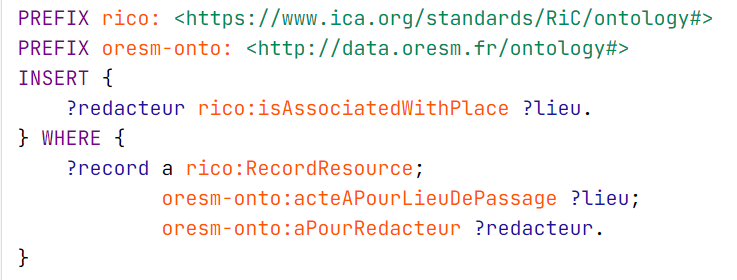
\includegraphics[width=0.9\linewidth]{images/insert redacteur.png}
    \caption{Requête SPARQL qui insère de nouveaux triplets dans le graphe en raisonnant sur le rédacteur et le lieu de passage d'un acte.}
    \label{fig:insert-redacteur}
\end{figure}